\documentclass{article}
\usepackage{geometry}
\geometry{a4paper,top=3cm,bottom=4cm,left=3.5cm,right=3.5cm,%
heightrounded,bindingoffset=5mm} %sistemiamo questi per decidere i bordi
\usepackage[utf8]{inputenc}
\usepackage{wrapfig}
\usepackage{float}
\usepackage{caption}
\usepackage[cc]{titlepic}
\usepackage{graphicx}
\usepackage{natbib}
\usepackage{graphicx}
\usepackage{color, colortbl}
\definecolor{Gray}{gray}{0.9}
\definecolor{LightCyan}{rgb}{0.88,1,1}
\usepackage[first=0,last=9]{lcg}
\newcommand{\ra}{\rand0.\arabic{rand}}
\begin{document}

\begin{titlepage}
	\centering
	
\includegraphics[width=0.80\textwidth]{marchio.jpg}\par\vspace{2cm}
	{\scshape\LARGE Data Mining Report \par}
	\vspace{1cm}
	{\scshape\Large Group 12 \\ \par}
	\vspace{1cm}
	{\huge\bfseries Analysis of car auctions\par}
	\vspace{2cm}
	{\Large\ Lorenzo Bellomo \\ Andrea Bruno \\ Marta Scalisi \\ Chiara Spampinato\par}
	\vspace{4cm}
    {\Large\ January 04, 2020\par}
	\end{titlepage}
	

	

\section{Data Understanding}
The data set contains information about car auctions. The majority of attributes give us information about vehicles. 
In this section we study our data, evaluate the quality of them, finding any missing values, invalid or misleading etc. in order to gain general insights about the data that will potentially be helpful for the complete analysis.

\subsection{Data Semantics}

\emph{RefId}: qualitative attribute which defines an unique ID number assigned to each vehicle\\
\emph{Auction}: categorical attribute which defines three different auction providers (Manheim, Adesa, other);\\
\emph{Make}: categorical attribute which gives us the name of the production company of the vehicle;\\
\emph{VehoDo}: numerical discrete attribute that points out the mileage;\\
\emph{Byrno}: categorical attribute that provides a buyer identifier which is made up of a sequence of numbers;\\
\emph{VNST}: categorical attribute that refers to a specific state where the car was purchased;\\
\emph{VehBCost}: continuous numerical attribute indicating the purchase price auction;\\
\emph{MMRA}: numerical attributes that define acquisition price of the vehicles, divided into:
\begin{itemize}
\item average condition price at time of purchase 
\item above average condition price at time of purchase
\item average condition price at time of purchase in the retail market
\item above average condition price at time of purchase in the retail market 
\end{itemize}

\emph{MMRC}: numerical attributes that define the current price of the vehicles, divided into:\\
\begin{itemize}
\item average condition price as of current day 
\item above condition price as of current day
\item above average condition price as of current day
\item above average condition  price as of current day in the retail market\\
\end{itemize}

Furthermore, analyzing the attributes there are two of them, Acquisition Type and Kickdate, which aren't in the dataset even though they are present in the dictionary.



\subsection{Assessing data quality}

We checked whether all the values of a specific attribute (VehYear, VehicleAge, VehOd, WarrantyCost) do belong to the domain of the consider attribute but we didn’t identified any errors.  For example VehOdo and WarrantyCost don’t contained mismatching values since 
none of them is $>=0$.

\begin{figure}[H]
	\centering
	\fbox{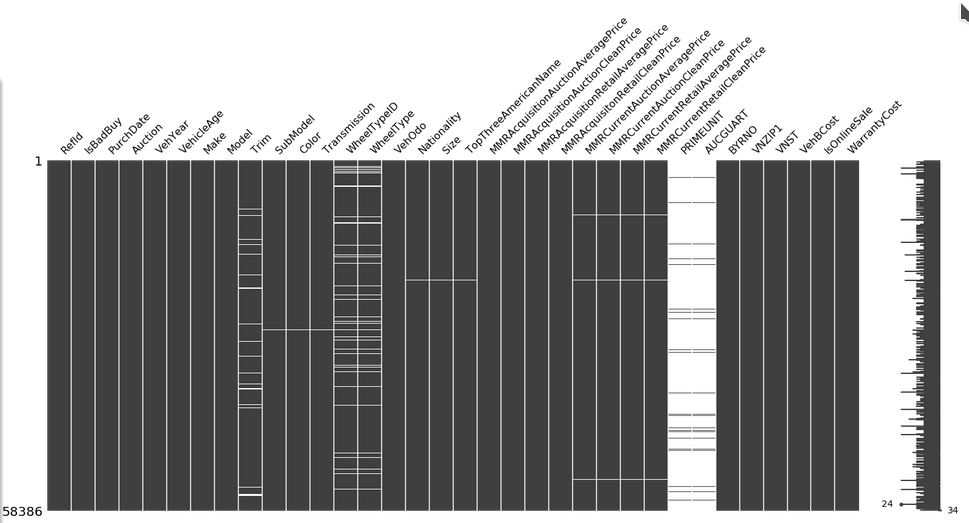
\includegraphics[width=.9\textwidth, height=.8\textheight, keepaspectratio]{missing.png}}
	\caption{{ Missing values }}
\end{figure}

After an analysis of missing values, we chose to correct them in this way: TRIM
LITERS
CYLINDERS
TRANSMISSION
PRICES
DOORS 
with the algorithm MICE (Multiple Imputation by Chained Equations) 




\subsection{Attributes Distribution}
In this section, we will analyze the distribution of some particular attributes, showing interesting statistic plots.
 

\begin{figure}[H]
	\centering
	\fbox{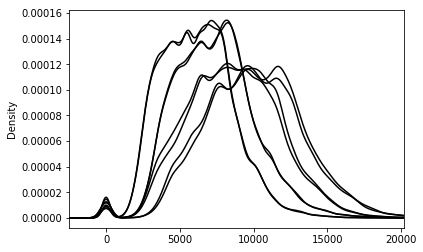
\includegraphics[width=.6\textwidth, height=.4\textheight, keepaspectratio]{index}}
	\caption{{ Distribution of 8 prices}}
\end{figure}

In the plot above we show the distribution of the 8 numerical attributes which point out the different prices of Vehicle as we explained in the first part of Data Semantics.  
    Analyzing the attribute \emph{VehBCost}, we can observe that Vehicles are usually sold for a price between 6000 and 7000, and a very low percentage of cars is sold above 11000 or below 5000 USD. (One of the most important attribute of our dataset).

 \begin{figure}[H]
	\centering
	\fbox{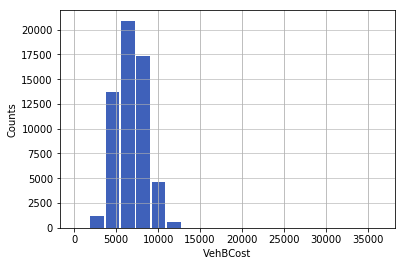
\includegraphics[width=.6\textwidth, height=.5\textheight, keepaspectratio]{hist.png}}
	\caption{{ Distribution of the attribute VehBCost}}
\end{figure}


For the attribute \emph{VSNT} we decide to plot the distribution on a map of the United States. By looking at the figure, it is possible to see that the major number of auctions is done in Texas (18800), followed by Florida (8317) and California (5673). On the other hand, the state with lower auctions is New York (4). Furthermore, there are no auctions in Montana, Wyoming, North Dakota, South Dakota, Kansas, Wisconsin, Maine, Vermont, Rhode Island and Connecticut. \\

\begin{figure}[H]
	\centering
	\fbox{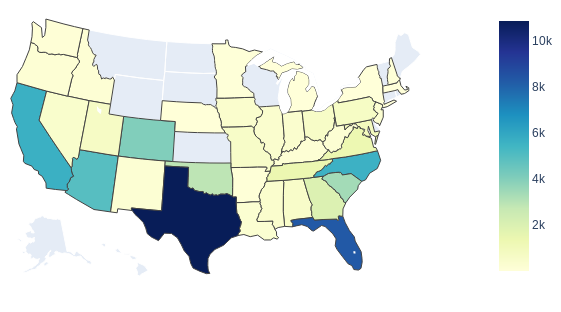
\includegraphics[width=.6\textwidth, height=.6\textheight, keepaspectratio]{newplot.png}}
	\caption{{ Distribution of the attribute VSNT}}
\end{figure}


As far as it concerns the attribute \emph{Color}, it is not surprising that the most common colors are blue, grey and white.
\begin{figure}[H]
    \centering
	\fbox{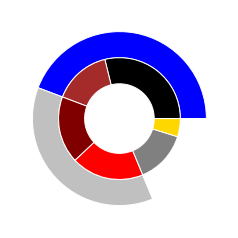
\includegraphics[width=.4\textwidth, height=.3\textheight, keepaspectratio]{color.png}}
	\caption{{ Distribution of the attribute Color}}
\end{figure}


\subsection{Variables Transformation and elimination of redundant variables}

We decided to split the attribute "Model" because, within it, too much information was contained. As a result, we use these information to create five different attributes:

\begin{itemize}
\item Engine Liters, 
\item NumCylinders,
\item 4X4, four-wheel drive
\item WheelDrive, others drive wheel configurations 
\item NumDoors, the number of the doors in a car
\end{itemize}

We also created three different attributes in order to separate the information contained in the variable "PurchDate" which specified the day the vehicle was sold into:

\begin{itemize}
\item PurchYear
\item PurchMonth
\item PurchDay
\item PurchWeekDay
\end{itemize}


\begin{figure}[H]
	\centering
	{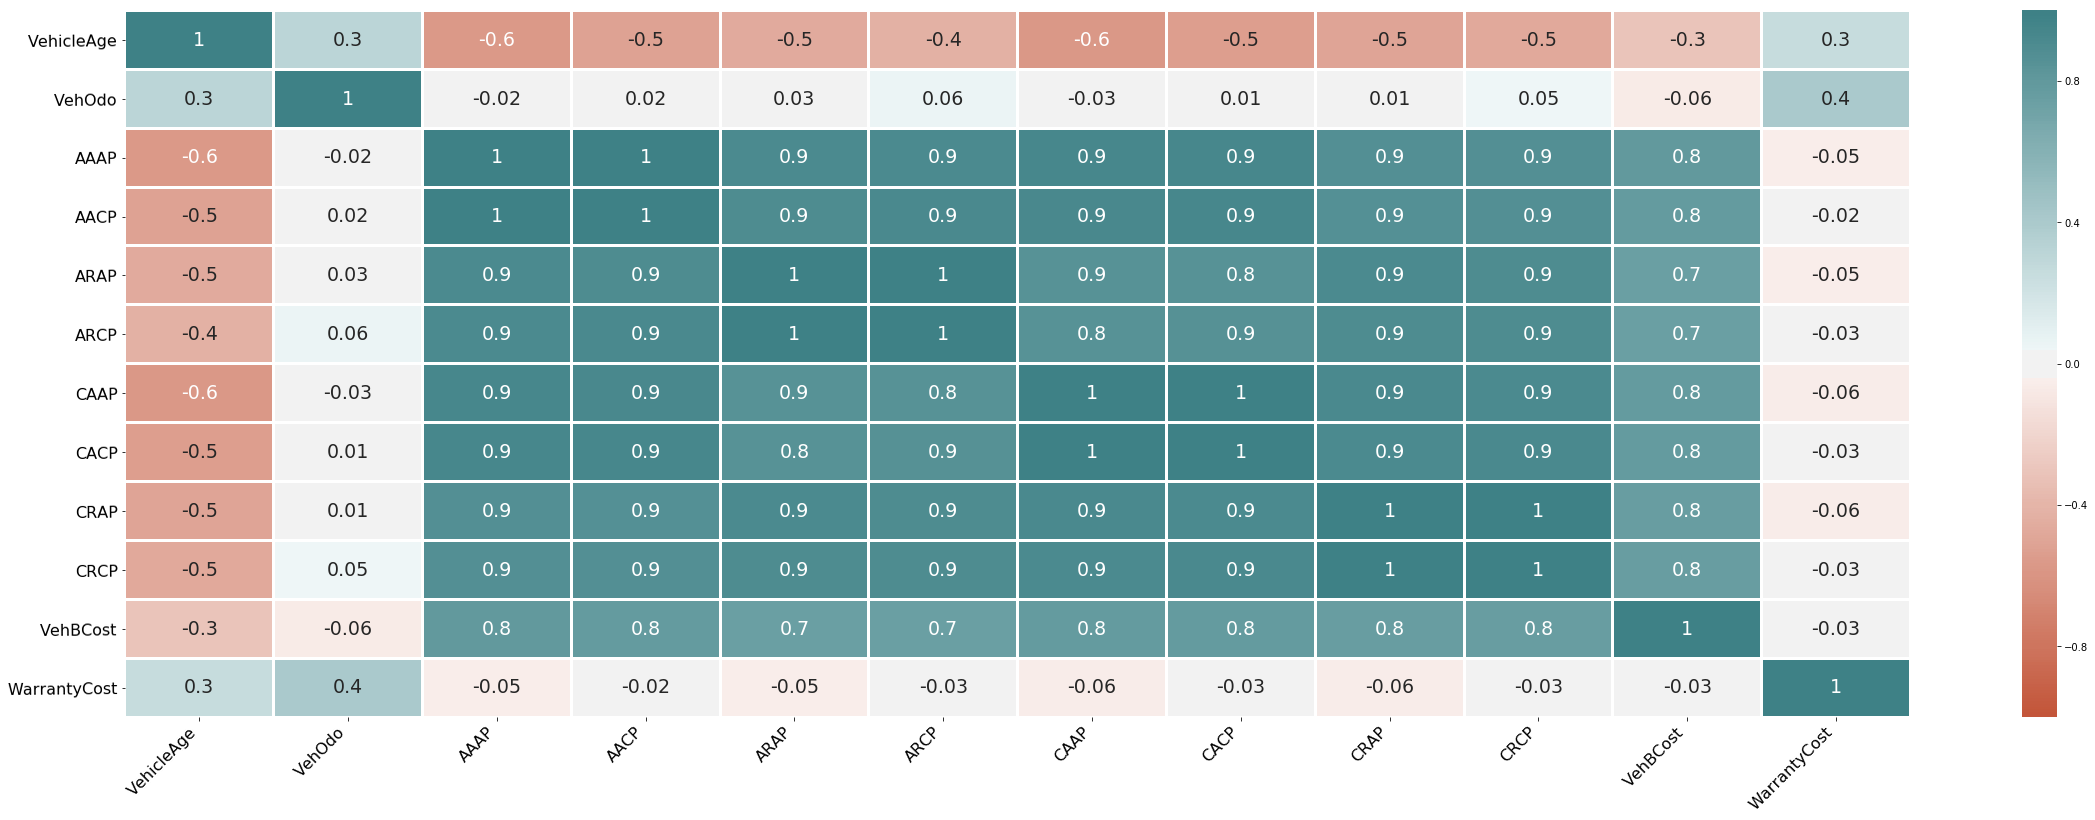
\includegraphics[width=1.1\textwidth, height=1.1\textheight, keepaspectratio]{corr.png}}
	\caption{{ Correlation matrix }}
\end{figure}
%ATTENZIONE ATTENZIONE! HO MESSO QUESTA SOLO PER REGOLARCI CON SPAZI E COSA DIRE


Finally, analyzing the correlation matrix of all the continuous attributes we can see that attributes MMRAcquisitionAuctionAveragePrice, MMRAcquisitionRetailAveragePrice, MMRCurrentAuctionAveragePrice, MMRCurrentRetailAveragePrice, MMRAcquisitionAuctionCleanPrice, MMRAcquisitonRetailCleanPrice, MMRCurrentAuctionCleanPrice, MMRCurrentRetailCleanPrice are strongly correlated. So, we reduce them in two attributes by use the algorithm PCA used to reduce the dimentionality of the date.
Le variabili sono diventate PCA1.

\section{Clustering}
In this section we describe the three Clustering algorithms applied to the data set (KMeans, DBScan and Hierarchical), and we describe the results

\subsection{Function Selection}
In K-means we tried to use both the \emph{MinMax} scaler and the standard \emph{z} scaler, observing that the clustering results were very similar. In the end, we decided to use the MinMax one.
In DBScan and Hierarchical we decided to adopt the Standard one because it gave us slightly better results.

\subsection{KMeans}
The following sections discuss the analysis of the results of KMeans clustering algorithm.

\subsection{Attributes' selection}
Considering that our dataset contains information about car auctions, we opt to study characteristics about cars, like how many kilometers the car has done (\textbf{VehOdo}), the auction selling price for the car (\textbf{VehBCost}), the cost of repairing or replacing previously sold products (\textbf{WarrantyCost}) and some samples of the different prices (\textbf{AAAP, ARAP}).

We created 5 Dataframes with these attributes in order to study which was the best combination of them.

\begin{table}[H]
\centering
\begin{tabular}{c|ccccccc}
\hline
 & Attributes set \\
\hline
\rowcolor{Gray}
1 & 'VehOdo' ,  'VehBCost',  'AAAP' \\
2 & 'WarrantyCost' , 'VehBCost' ,  'AAAP'  \\
\rowcolor{Gray}
3 & 'AAAP' ,  'ARAP' ,  'VehBCost' \\
4 & 'WarrantyCost' ,  'VehOdo' ,  'VehBCost'  \\
\rowcolor{Gray}
5 & 'WarrantyCost' ,  'AAAP' , 'VehOdo' \\
    \end{tabular}
    \end{table}


\subsubsection{Identification of best k}

    
In order to pick the best parameter k for K-Means, we made use of the Knee method by computing the SSE for K $\in$ [2,16]. The best SSE was obtained in the Data Frame 3, which was originally chosen for his highest correlation among the attributes.

However, when we tried plotting the data, we did not obtain any interesting information in order to better interpreter the data behaviour. We then decided to give up the best SSE by choosing the Data Frame 4 which has a lower SSE but semantically more interesting results.


\begin{figure}[H]
	\centering
	\includegraphics[width=.49\textwidth]{cattura}\hfill
	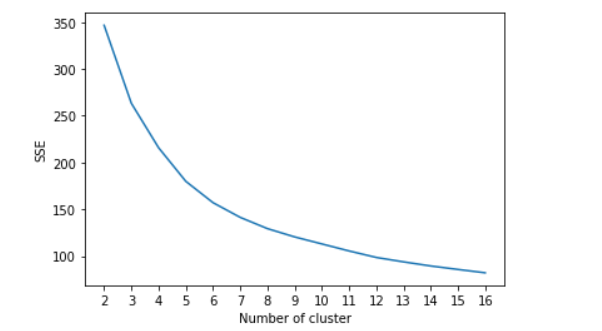
\includegraphics[width=.49\textwidth]{SSE2}\hfill
	\caption{Plot SSE of Attribute set 3 (left) and 4 (right).}
	\label{fig:KmeansSSE}
\end{figure}
From those plot, we 

We noticed that the SSE curves for the 5 data frames share a strong similarity (same curvature, but different SSE). Their behaviour is very similar to the ones shown in figure \ref{fig:KmeansSSE}, and we found, using the \emph{knee method}, that the best attribute \emph{k} for all the data frames was 6. All the values collected for the the different data frames are shown in table \ref{tab:SSESilu}. In particular, the lowest SSE is by far the one of data frame 3. \\However, we decided to discard this result since the 6 cluster found by the algorithm were basically groups of cars in different price ranges. We decided that the best clustering, both semantically and parameter wise, was the DF4 one (taking in consideration 'WarrantyCost', 'VehOdo' and 'VehBCost').

\begin{table}[H]
\centering
\begin{tabular}{c|ccccccc}
\hline
 &  Best k & SSE& Silhouette \\
\hline
\rowcolor{Gray}
DF1 & 6 & 106.0 & 0.309 \\
DF2 & 6 & 90.0 & 0.307  \\
\rowcolor{Gray}
DF3 & 6 & 40.0 & 0.294 \\
DF4 & 6 & 157.0 & 0.287  \\
\rowcolor{Gray}
DF5 & 6 & 184.0\textbf & 0.278 \\
    \end{tabular}
    	\caption{{ Summary of the SSE, Silhouette and k values obtained for all the Attribute sets with K-means}}
    \label{tab:SSESilu}
    \end{table}


\subsubsection{Description of the best clustering}
\label{sec:cluster}
The following descriptions refer to the results of the clustering that was proposed as the best in previous section. Every result is presented with its centroid, that describes the core point of the cluster, and a textual interpretation of the kind of cars that are present in those clusters. 
The centroids coordinates are expressed like this:  
$$ \mathbf{centroid} = (\mathbf{VehBCost}, \mathbf{WarrantyCost}, \mathbf{VehOdo}) $$
In figure \ref{fig:centroid} the clustering results are shown plotted in 2 dimensions (WarrantyCost and VehOdo). The plot does not show the third dimension (VehBCost) because, from the results, this latter one results the least important dimension (as it will be evident from the centroids shown when describing the clusters). The figure also shows the cluster centroids with a star on the plot. 

\begin{figure}[H]
    \centering
	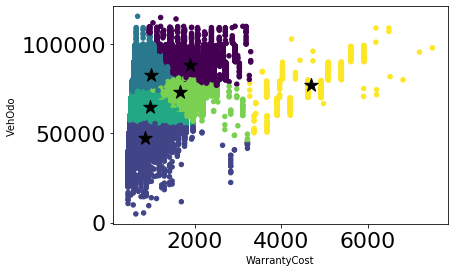
\includegraphics[width=.8\textwidth, keepaspectratio]{centroid}
	\caption{{Clusters plotted with WarrantyCost and VehOdo}}
	\label{fig:centroid}
\end{figure}

The clusters descriptions for figure \ref{fig:centroid} are:
\begin{enumerate}
    \item $\mathbf{centroid}: (6\,500,  1\,900,  88\,000)$: cars with very high odometer reading and pretty high warranty cost (purple cluster). Those cars are sold for a price which is in line with the mean of the prices.
    \item $\mathbf{centroid}: (6\,800,  850,  48\,000)$: cars which are pretty new , with low  reading and low warranty cost (light blue cluster). As expected their cost is slightly above average.
    \item $\mathbf{centroid}: (6\,400,  1\,000,  83\,000)$: cars with high odometer reading but low warranty cost (azure cluster). Those cars are probably considered to be solid (low outage risk) even after years of use, and are sold at a normal price.
    \item $\mathbf{centroid}: (6\,700,  1\,000,  65\,000)$: cars with low warranty cost and average odometer (aquamarine cluster). There is not much to say about this cluster, as it represents the average car.
    \item $\mathbf{centroid}: (7\,300,  1\,700,  73\,000)$: Cars with high warranty cost, but average odometer reading (green cluster). This is one of the more interesting cluster, as it shows that relatively high risk cars are sold at a price which is higher than expected (considering high warranty cost as a sign of risk).
    \item $\mathbf{centroid}: (5\,300,  4\,700,  77\,000)$: Exceptionally high warranty cost, high odometer reading (yellow cluster). This cluster is the least populated one, and the most sparse one. It homes those very risky buys, and in addition to that, cars in this cluster are also pretty dated. They are sold, as expected, at a very low price. 
\end{enumerate}
Given this results, we tried to understand if bad buys were located mainly in one of those clusters. By plotting this information in figure \ref{fig:clusterbuy}, we noticed that cluster 2 (new cars with low odometer reading), has the least amount of bad buys.
\begin{figure}[H]
    \centering
	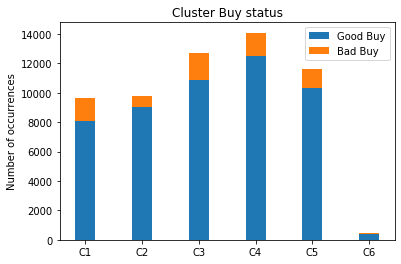
\includegraphics[width=.7\textwidth, keepaspectratio]{clusterbuy}
	\caption{{Distribution of IsBadBuy with respect to the 6 clusters found}}
	\label{fig:clusterbuy}
\end{figure}




\subsection{DB Scan}
In this section, we explain the approach used to generate clusters with DBscan algorithm.

\subsubsection{Attributes and distance function}
We decided, following the same reasoning we used for \emph{KMeans}, to attempt clustering over the same set of attributes. We also decided to use euclidean distance, and Z-Score scaling for the data frame.\\
The results shown in the following sections are only relative to the data frame with columns 'VehOdo0, 'VehBCost' and 'WarrantyCost' (the same data frame used for KMeans). Other possible attributes choices did not change much the final result, so we decided that using the same attributes allows us to more easily see the difference between the two algorithms.

\subsubsection{Study of the clustering parameters}
In order to choose the right $\epsilon$ and $\mathbf{min points}$, we adopted the knee method by plotting the distance to the \emph{k-th} nearest neighbour, where k was taken from [32, 64, 128, 256, 512]. The resulting curves, shown in figure \ref{fig:kth}, were used to select the right epsilon for attempting the clustering with DB-Scan. 
\begin{figure}[H]
\centering
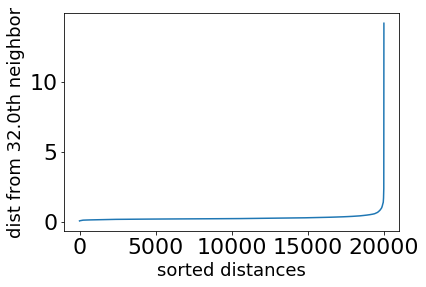
\includegraphics[width=.32\textwidth]{a32}\hfill
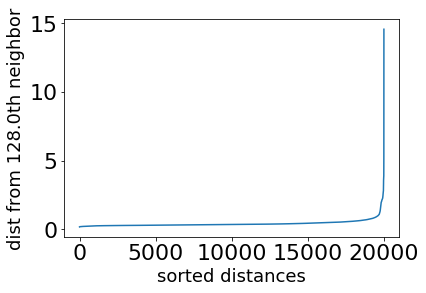
\includegraphics[width=.32\textwidth]{a128}\hfill
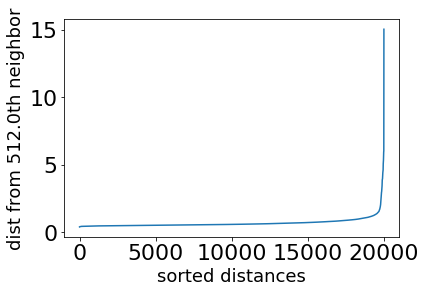
\includegraphics[width=.32\textwidth]{a512}
\caption{k-th neighbour distance, with k = 32, k = 128, k = 512}
\label{fig:kth}
\end{figure}
Given those plots, we chose epsilon as shown in table \ref{tab:kth}.
It is important to know, however, that this approach failed for reasons described in section \ref{sec:dbscaneval}, so another set of attributes with more interesting results is shown in table \ref{tab:dbscan}. Those values were found by brute force, by attempting, for all k shown in the list before, $ \epsilon = 0.1, 0.11, 0.12\dots 0.8$, and visually inspecting the results.\\

\begin{table}
\parbox{.45\linewidth}{
\centering
\begin{tabular}{c|c}
\hline
min points & $\epsilon$\\
\hline
\rowcolor{Gray}
32 & 0.75 \\
64 & 0.95 \\
\rowcolor{Gray}
128 & 1.22 \\
256 & 1.36 \\
\rowcolor{Gray}
512 & 1.64 \\
\end{tabular}
\caption{K-th nearest neighbours parameters}
\label{tab:kth}
}
\hfill
\parbox{.45\linewidth}{
\centering
\begin{tabular}{c|c}
\hline
min points & $\epsilon$\\
\hline
\rowcolor{Gray}
32 & 0.17 \\
64 & 0.22 \\
\rowcolor{Gray}
128 & 0.29 \\
256 & 0.38 \\
\rowcolor{Gray}
512 & 0.48 \\
\end{tabular}
\caption{Manually found parameters}
\label{tab:dbscan}
}
\end{table}

\subsubsection{Characterization and interpretation of the obtained clusters}
\label{sec:dbscaneval}
First, we are going to analyze the results with parameters shown in table \ref{tab:kth}. The result was that of a single cluster, containing all the points in the data set, with the exception of $\sim 100$ elements, which were labeled as noise points. This is because the data forms one big cloud of points, with different density distribution inside. This kind of behaviour represents the conditions under which DB scan performs worst, and this is the reason why the \emph{k-th} neighbour distance approach failed. \\
We then decided to try and find the most dense areas in the data set, by manually checking a lot of configurations. This approach, however, does not find cluster, but only finds highly populated areas in the data set. 
The best results were found when the number of noise points was close to half the total amount in the data set. Those results correspond to the ones found with the parameters shown in table \ref{tab:dbscan} and some example of such clustering is shown in figure \ref{fig:dbscan}.

\begin{figure}[H]
\centering
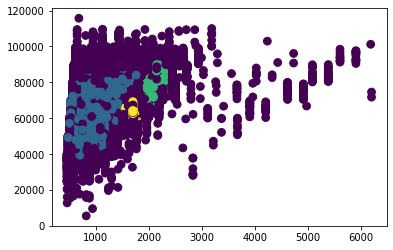
\includegraphics[width=.49\textwidth]{cazzo}\hfill
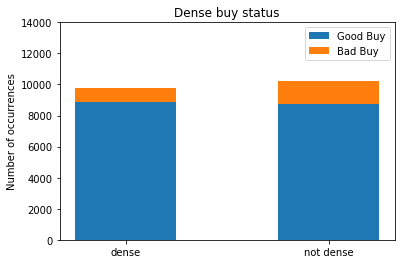
\includegraphics[width=.49\textwidth]{bigboi}\hfill
\caption{DBScan clustering results with $\mathbf{minpoints} = 256$ and $\epsilon = 0.38$. Purple colors are noise points}
\label{fig:dbscan}
\end{figure}

We realised that most of the cars sold have $50\,000 \sim 70\,000$ odometer reading when sold, and denser areas have slightly less bad buys overall. \\
Having said that, DBscan is the algorithm that performs the worst on this data set.

\subsection{Hierarchical Clustering}
In this section, we explain the approach used to generate clusters with Hierarchical algorithm.
\subsubsection{Attribute Choices}
We decided to perform clustering on the following attributes set:
\begin{enumerate}
    \item 'VehOdo', 'VehBCost', 'AAAP'
    \item 'WarrantyCost', 'VehBCost', 'VehOdo'
\end{enumerate}

\subsubsection{Algorithms and Dendrograms}
\label{sec:hier}
We decided to perform clustering with euclidean and manhattan distance as metrics, and to perform, for each of those metrics ward, single, complete and average linkages (with the exception of manhattan distance with ward linkage, since it is not allowed).\\
For each one of those results, we attempted clustering with $\mathbf{numberOfCluster} \in [2, 10]$, and computed the silhouettes for all the results.
Figure \ref{fig:silu} shows the silhouettes for the results found with all the algorithms on data frame 2 (the same used for KMeans and DBScan).
\begin{figure}[H]
\centering
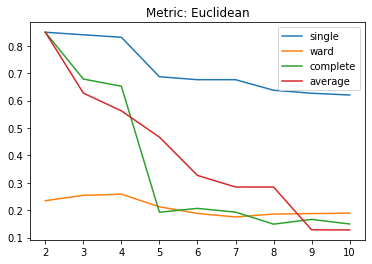
\includegraphics[width=.49\textwidth]{silueuc}\hfill
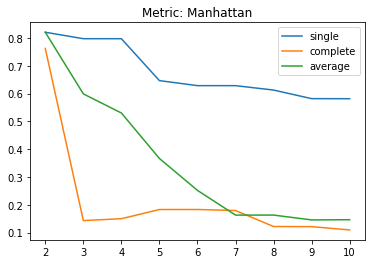
\includegraphics[width=.49\textwidth]{siluman.png}\hfill
\caption{Silhouettes for all algorithms and all metrics on data frame 2}
\label{fig:silu}
\end{figure}
From those plot, we notice a tendency for the silhouette to drop when the number of cluster passes from 4 to 5. We then decide to perform clustering with 4 clusters.
Given that, we visually inspected the results and found that the only ones with interesting clusters are:
\begin{itemize}
    \item Euclidean metric and ward linkage
    \item Manhattan metric and complete linkage
\end{itemize}
The visual result of those clustering is shown in figure \ref{fig:hier}, while their respective dendrograms are shown in figure \ref{fig:dend}. All the other clustering attempts produced highly imbalanced cluster (one main cluster and some single digit size clusters).
\begin{figure}[H]
\centering
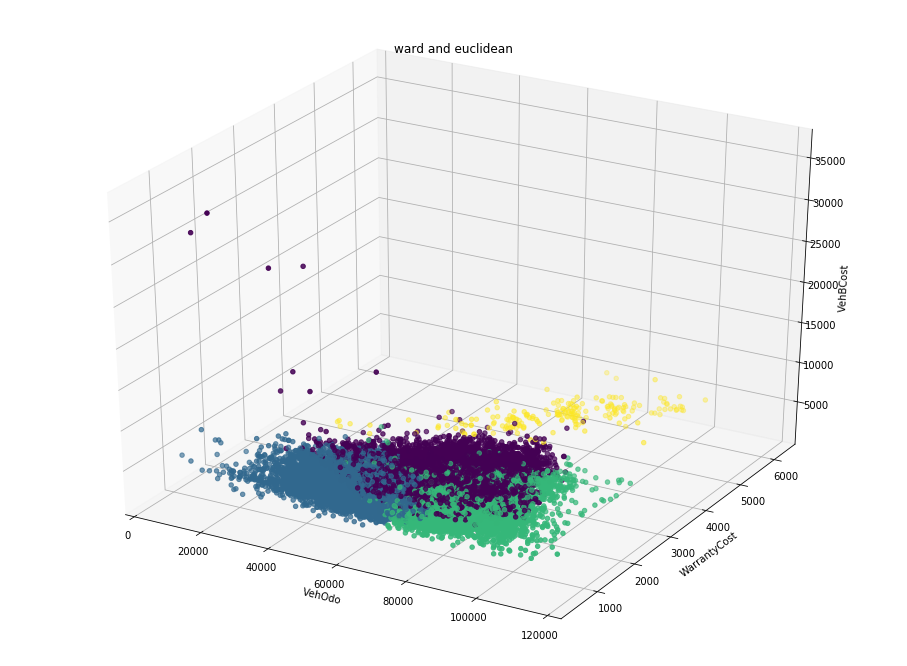
\includegraphics[width=.49\textwidth]{wardeucl}\hfill
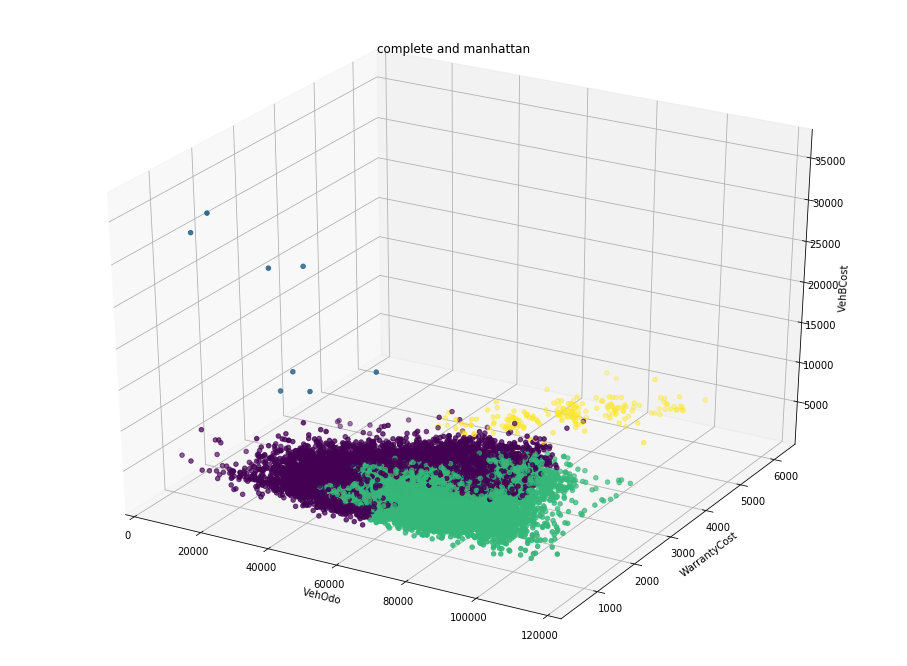
\includegraphics[width=.49\textwidth]{complman}\hfill
\caption{Hierarchical clustering results, number of clusters is 4}
\label{fig:hier}
\end{figure}
\begin{figure}[H]
\centering
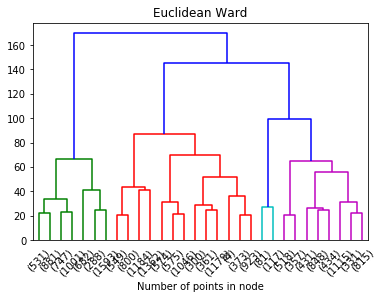
\includegraphics[width=.49\textwidth]{dendeuc}\hfill
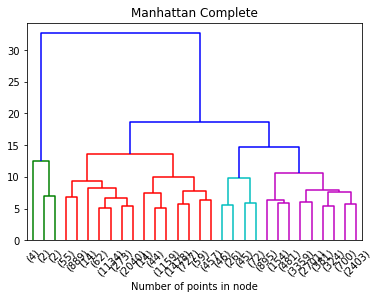
\includegraphics[width=.49\textwidth]{dendman}\hfill
\caption{Dendrograms plotted with \emph{lastp} truncate mode}
\label{fig:dend}
\end{figure}


\subsubsection{Best clustering approach and comparison of the clustering obtained}
In conclusion, the best clustering results were found in the circumstances shown in section \ref{sec:hier}. The results, semantically speaking, highly resemble the ones found using KMeans. Both results find a cluster in the high warranty cost cars (displayed in both figure \ref{fig:hier} and in figure \ref{fig:centroid} for KMeans, where the highlighted cluster is displayed in yellow).\\
The main difference is in the way that points in the "big cloud" are assigned a cluster. The reasoning, anyway, is really similar to the one made in section \ref{sec:cluster} regarding KMeans, so we refer to that one.



\section{Classification}

Todo ANDREA QUI!!!!



\section{Pattern Mining}
In this section we try to find the best pattern and association rules in order to better understand the information hidden in the dataset. 

\section{Conclusion}
buongiornissimo!!!! kafffeeeeeee!??!???!?!??!


\end{document}


